
\begin{figure}
\begin{center}
\caption{Introduzco mi nombre y usuario de la ugr, con contraseña "Swap1234"  durante la instalación de la máquina virtual m1-anabuenrua}
\label{instalacion_nombre}
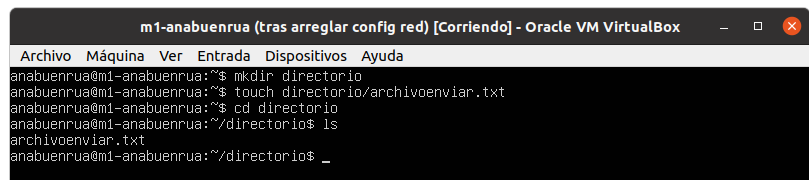
\includegraphics[scale=0.5]{enviar_1}
\end{center}
\end{figure}


\chapter{Copia de archivos}

Vamos a comenzar enviando el directorio con \verb|tar|, de forma simple. Comenzamos creando un directorio con un archivo como se ve en \eqref{enviar_1}.

\begin{figure}
\begin{center}
\caption{Creación de directorio con un archivo en m1 y contenido de este archivo.}
\label{enviar_1}
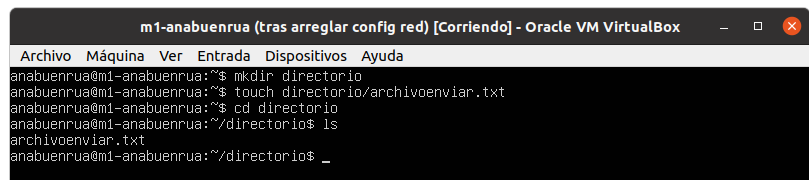
\includegraphics[scale=0.5]{enviar_1}
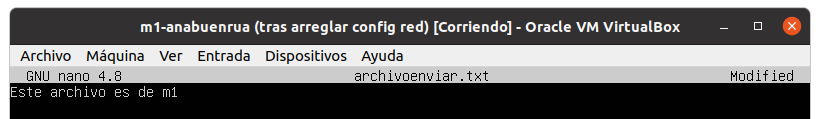
\includegraphics[scale=0.5]{enviar_2}
\end{center}
\end{figure}

Y mandamos el directorio comprimido con tar \eqref{enviar_3}. Como ya configuramos el acceso por ssh sin contraseña no nos la pide.

\begin{figure}
\begin{center}
\caption{Envío del archivo comprimido con tar}
\label{enviar_3}
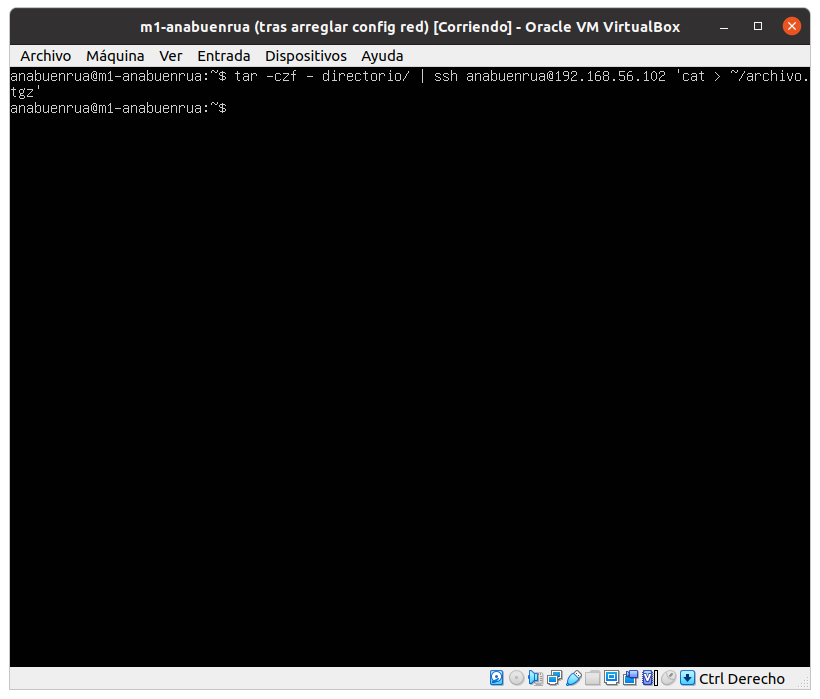
\includegraphics[scale=0.5]{enviar_3}
\end{center}
\end{figure}

Finalmente descomprimimos y comprobamos que se ha mandado correctamente \eqref{enviar_4}.

\begin{figure}
\begin{center}
\caption{Descompresión y comprobación del envío correcto del archivo.}
\label{enviar_4}
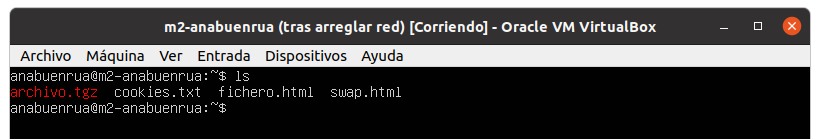
\includegraphics[scale=0.5]{enviar_4}
\end{center}
\end{figure}

\section{Envío mediante tar y scp}

Ahora vamos a enviarlo mediante tar y scp. Para ello creamos el tar y lo mandamos mediante scp como se ve en \eqref{enviar_6}

\begin{figure}
\begin{center}
\caption{Compresión con tar y envío mediante scp}
\label{enviar_6}
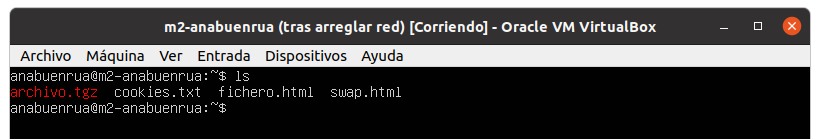
\includegraphics[scale=0.5]{enviar_4}
\end{center}
\end{figure}

Comprobamos en \eqref{enviar_7} que en la máquina 2 se encuentra directorio2.

\begin{figure}
\begin{center}
\caption{Comprobación de la llegada de directorio2 a m2}
\label{enviar_7}
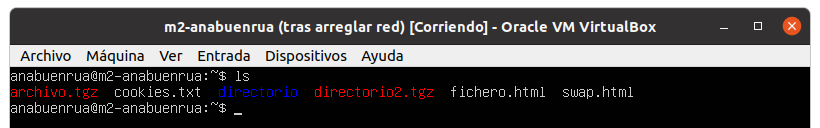
\includegraphics[scale=0.5]{enviar_7}
\end{center}
\end{figure}

\section{Comandos avanzados}

Vamos a enviar el directorio esta vez usando scp y algunas de sus opciones.

Comenzamos son \verb|-r|, que copia recursivamente directorios enteros, y \verb|-v| nos da información de la copia y de ssh. Como vemos en \eqref{enviar_8} muestra mucha información.

\begin{figure}
\begin{center}
\caption{Uso de scp con comandos avanzados}
\label{enviar_8}
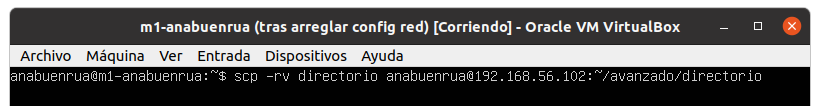
\includegraphics[scale=0.5]{enviar_8}
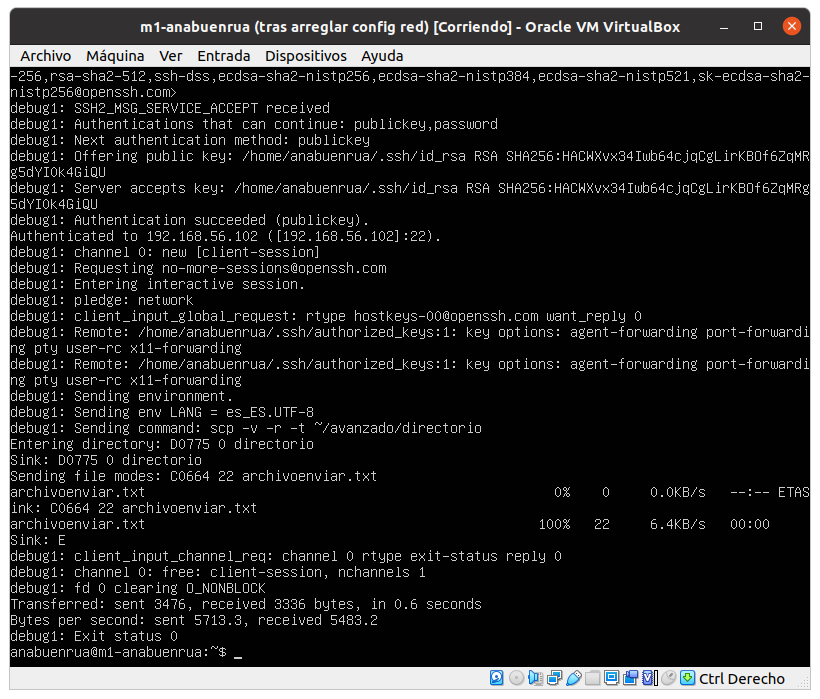
\includegraphics[scale=0.5]{enviar_9}
\end{center}
\end{figure}

También podemos usar la opción \verb|-q| que desactiva que se muestren mensajes por si se mandan muchos archivos \eqref{enviar_11}

\begin{figure}
\begin{center}
\caption{Uso de scp con comandos avanzados}
\label{enviar_11}
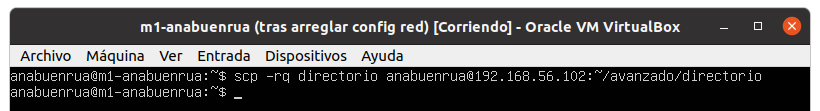
\includegraphics[scale=0.5]{enviar_11}
\end{center}
\end{figure}

Finalmente, con \verb|-P| podemos indicar el puerto. Por ejemplo de m2 a m1 como se muestra en \eqref{enviar_13}

\begin{figure}
\begin{center}
\caption{Uso de scp con comandos avanzados}
\label{enviar_13}
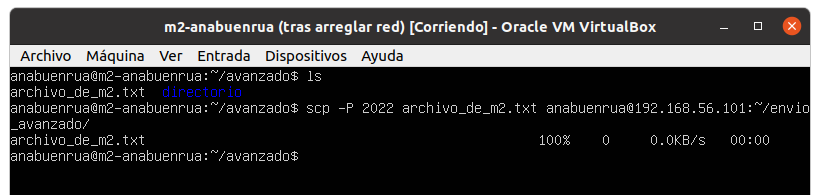
\includegraphics[scale=0.5]{enviar_13}
\end{center}
\end{figure}


\chapter{Utilizando Rsync}

Rsync ya está instalado en ambas máquinas, comprobamos su versión en \eqref{rsync_1}

\begin{figure}
\begin{center}
\caption{Comprobación de la versión de Rsync.}
\label{rsync_1}
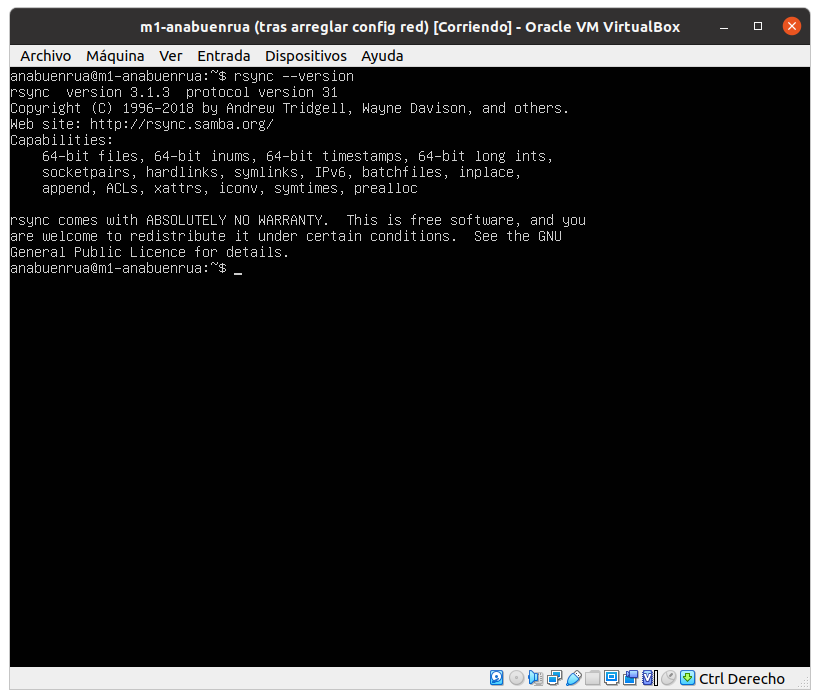
\includegraphics[scale=0.5]{rsync_1}
\end{center}
\end{figure}

Con chown cambiamos el propietario de la carpeta \verb|var/www/| ejecutando el comando \eqref{rsync_2}

\begin{figure}
\begin{center}
\caption{Cambiamos el propietario de la carpeta /var/www/}
\label{rsync_2}
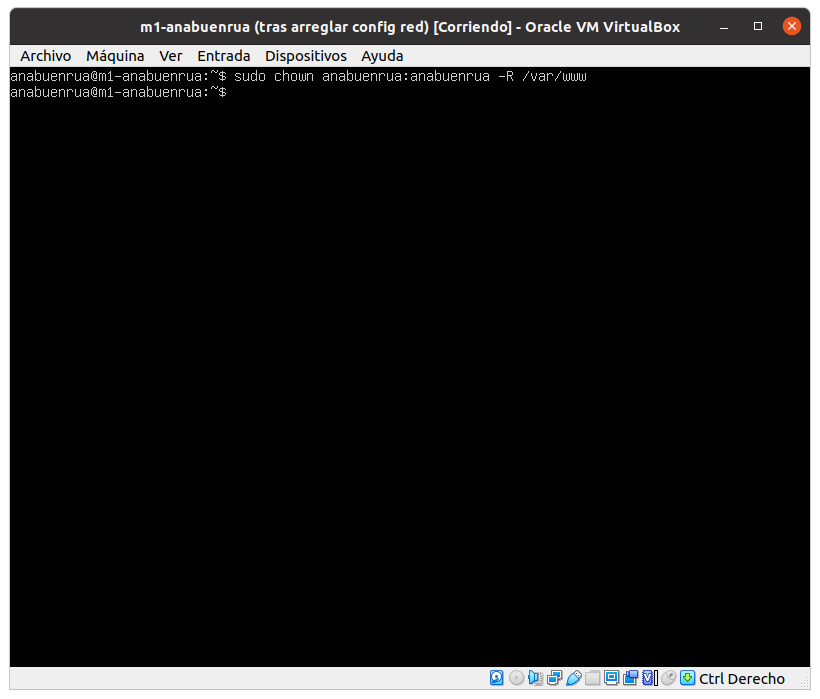
\includegraphics[scale=0.5]{rsync_2}
\end{center}
\end{figure}

Y ejecutamos rsync en m1, para copiar los archivos a m2, como se muestra en \eqref{rsync_4}:

\begin{figure}
\begin{center}
\caption{Sincronización de la carpeta /var/www/ de m1 a m2}
\label{rsync_4}
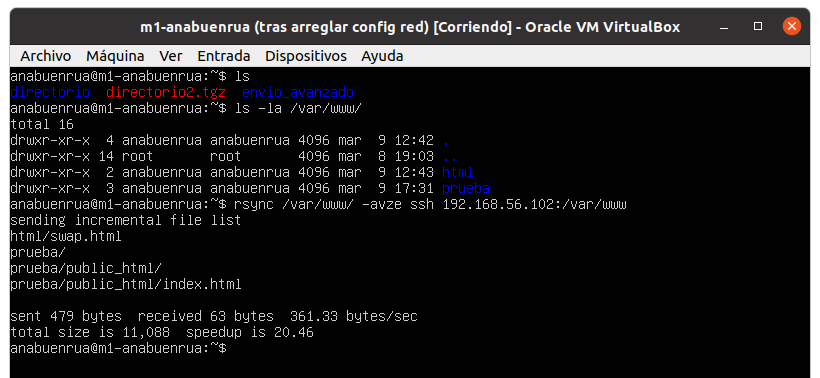
\includegraphics[scale=0.5]{rsync_4}
\end{center}
\end{figure}

Las opciones usadas son \verb|-a|, que indica recursividad (archive), \verb|-e| especifica el shell remoto que se va a utilizar, \verb|-v| es verbose, para dar más información y \verb|-z| para comprimir los archivos durante la trasnferencia.

\section{Opciones avanzadas}

Como opciones avanzadas vamos a usar \verb|--stats|, que nos muestra estadísticas, \verb|--exclude|, para excluir carpetas o directorios, \verb|--delete|, para borrar en la máquina destino los ficheros borrados de la máquina origen y \verb|--dry-run|, que permite a rsync hacer un "clonado de prueba", de forma que podemos ver lo que se va a clonar pero sin llegar a efectuarse la copia.

Comenzamos creando un directorio de prueba a clonar desde m1 a m2 \eqref{rsync_a1}.

\begin{figure}
\begin{center}
\caption{Creamos directorio de prueba para clonar usando rsync.}
\label{rsync_a1}
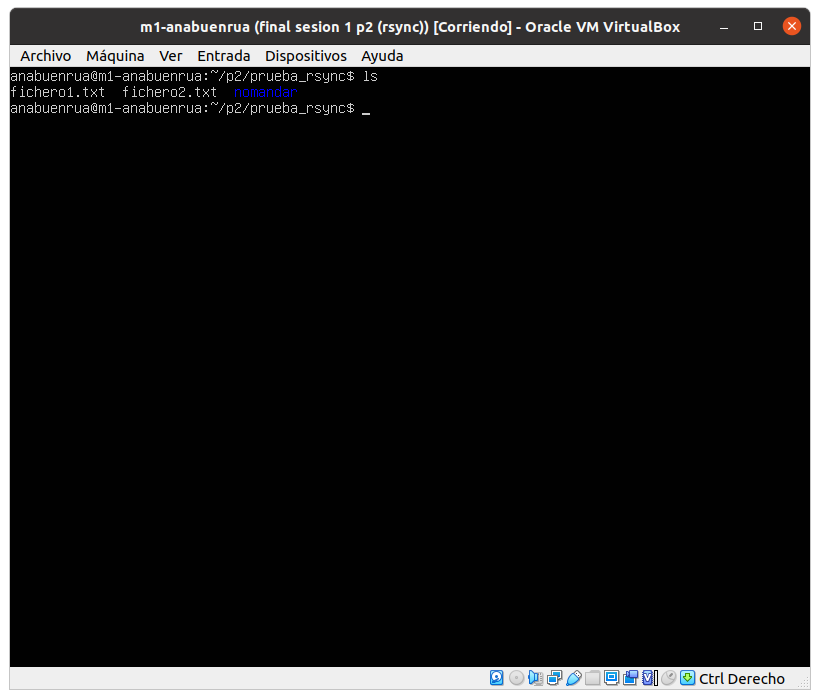
\includegraphics[scale=0.5]{rsync_a1}
\end{center}
\end{figure}

Comenzamos realizando una prueba de lo que sería la copia con \verb|--dry-run|, como mostramos en \eqref{rsync_a2}.

\begin{figure}
\begin{center}
\caption{Ejecución de rsync don --dry-run}
\label{rsync_a2}
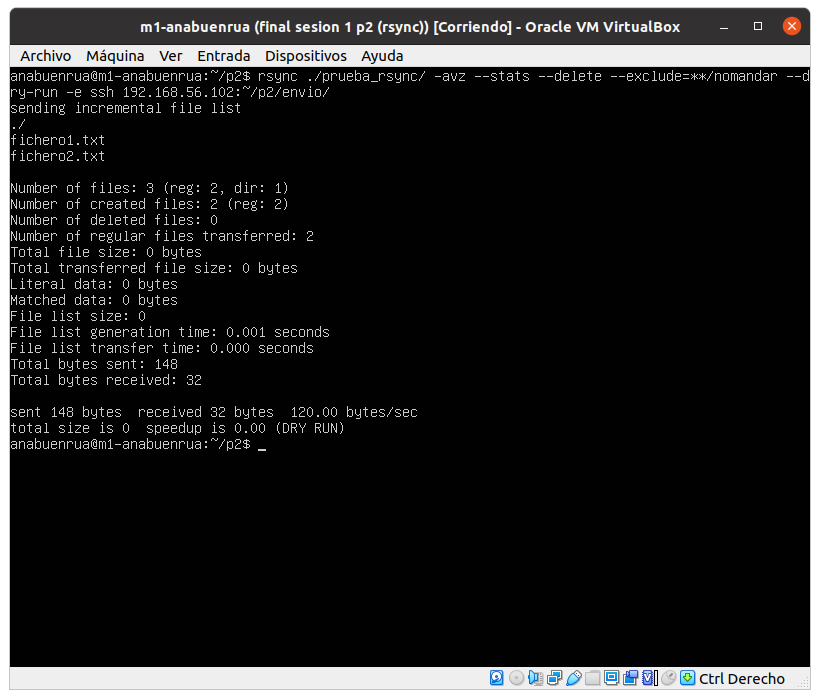
\includegraphics[scale=0.5]{rsync_a2}
\end{center}
\end{figure}

Así, comprobamos que en efecto se va a mandar lo que queremos, pero todavía no hemos clonado nada, como podemos comprobar en la máquina m2, se puede ver en \eqref{rsync_a3}

\begin{figure}
\begin{center}
\caption{Estado de m2 tras la ejecución de rsync con --dry-run}
\label{rsync_a3}
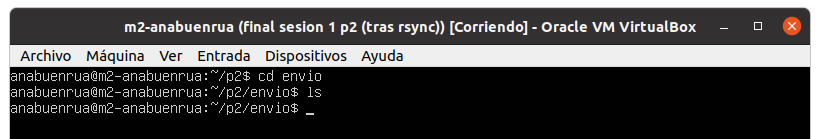
\includegraphics[scale=0.5]{rsync_a3}
\end{center}
\end{figure}

Ahora sí, procedemos a realizar el envío quitando la opción \verb|--dry-run|, en \eqref{rsync_a4}, y comprobamos que se ha copiado con éxito en \eqref{rsync_a5}

\begin{figure}
\begin{center}
\caption{Ejecución de rsync con opciones avanzadas.}
\label{rsync_a4}
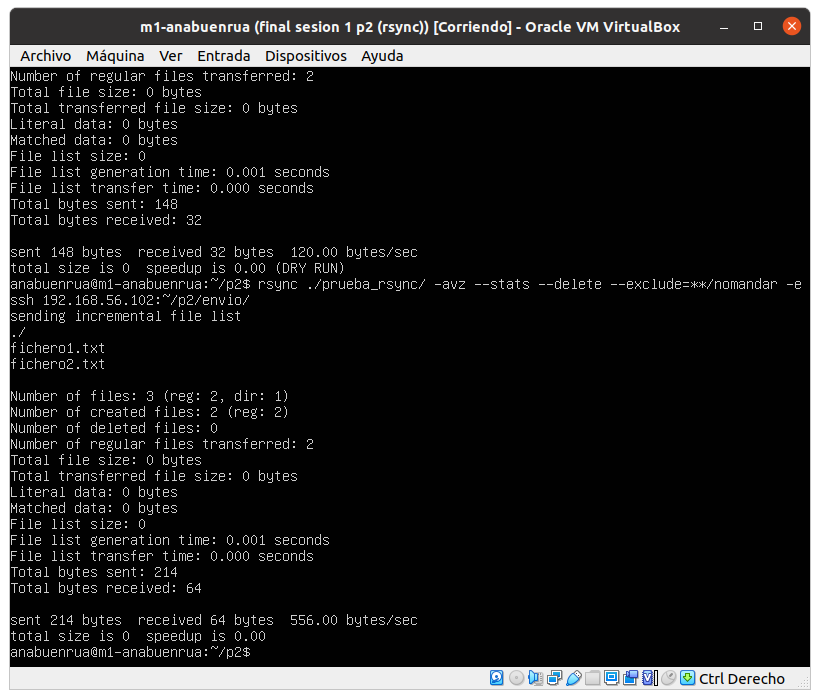
\includegraphics[scale=0.5]{rsync_a4}
\end{center}
\end{figure}

\begin{figure}
\begin{center}
\caption{Comprobando la copia correcta de los ficheros en m2.}
\label{rsync_a5}
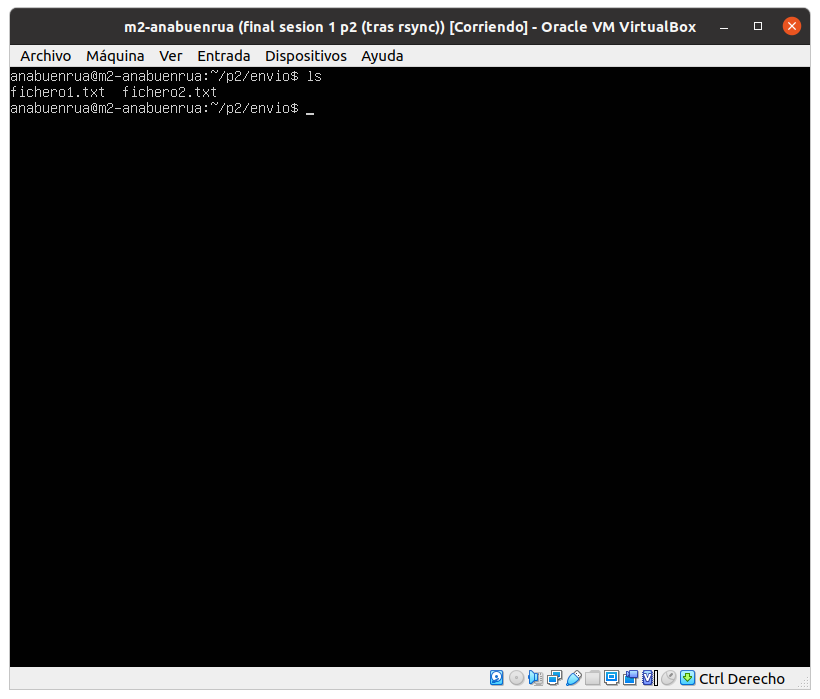
\includegraphics[scale=0.5]{rsync_a5}
\end{center}
\end{figure}

Es claro que el argumento \verb|--exclude| ha evitado que se copie el directorio \verb|nomandar|.

Finalmente, probamos a eliminar el fichero \verb|fichero1.txt| y repetir el clonado, comprobando así que la opción \verb|--delete| lo elimina en m2 también, como se ve en \eqref{rsync_a6}

\begin{figure}
\begin{center}
\caption{Ejecución de rsync tras borrar fichero1 en m1 y el resultado en m2}
\label{rsync_a6}
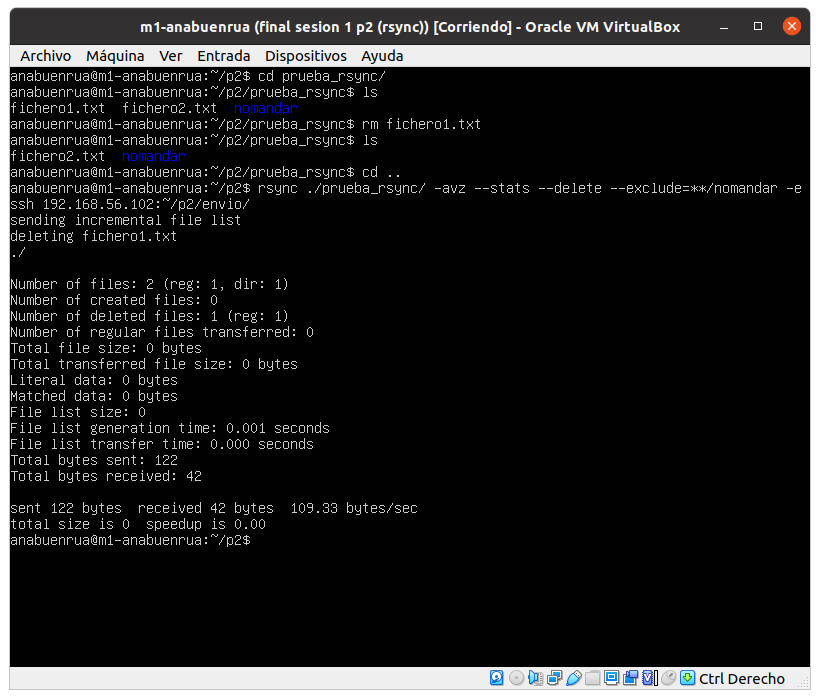
\includegraphics[scale=0.5]{rsync_a6}
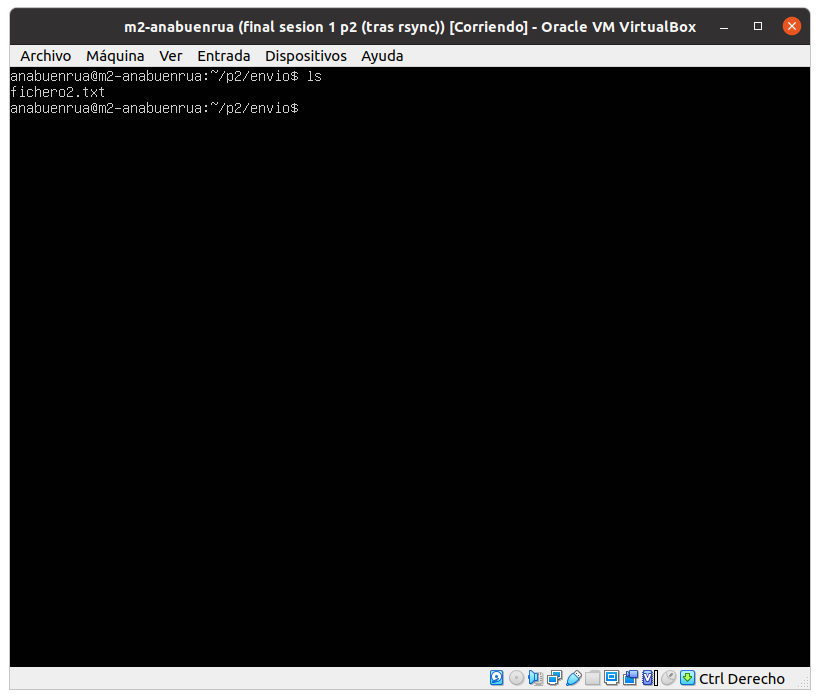
\includegraphics[scale=0.5]{rsync_a7}
\end{center}
\end{figure}







